\documentclass[journal,12pt,twocolumn]{IEEEtran}
%

\usepackage{setspace}
\usepackage{gensymb}
\singlespacing

\usepackage{amsmath}
\usepackage{amsthm}
\usepackage{txfonts}
\usepackage{cite}
\usepackage{enumitem}
\usepackage{mathtools}
\usepackage{listings}
    \usepackage{color}                                            %%
    \usepackage{array}                                            %%
    \usepackage{longtable}                                        %%
    \usepackage{calc}                                             %%
    \usepackage{multirow}                                         %%
    \usepackage{hhline}                                           %%
    \usepackage{ifthen}                                           %%
  %optionally (for landscape tables embedded in another document): %%
    \usepackage{lscape}     
\usepackage{multicol}
\usepackage{chngcntr}
\renewcommand\thesection{\arabic{section}}
\renewcommand\thesubsection{\thesection.\arabic{subsection}}
\renewcommand\thesubsubsection{\thesubsection.\arabic{subsubsection}}

\renewcommand\thesectiondis{\arabic{section}}
\renewcommand\thesubsectiondis{\thesectiondis.\arabic{subsection}}
\renewcommand\thesubsubsectiondis{\thesubsectiondis.\arabic{subsubsection}}

% correct bad hyphenation here
\hyphenation{op-tical net-works semi-conduc-tor}
\def\inputGnumericTable{}                                 %%

\lstset{
%language=C,
frame=single, 
breaklines=true,
columns=fullflexible
}

\begin{document}
%


\newtheorem{theorem}{Theorem}[section]
\newtheorem{problem}{Problem}
\newtheorem{proposition}{Proposition}[section]
\newtheorem{lemma}{Lemma}[section]
\newtheorem{corollary}[theorem]{Corollary}
\newtheorem{example}{Example}[section]
\newtheorem{definition}[problem]{Definition}
\newcommand{\BEQA}{\begin{eqnarray}}
\newcommand{\EEQA}{\end{eqnarray}}
\newcommand{\define}{\stackrel{\triangle}{=}}

\bibliographystyle{IEEEtran}


\providecommand{\mbf}{\mathbf}
\providecommand{\pr}[1]{\ensuremath{\Pr\left(#1\right)}}
\providecommand{\qfunc}[1]{\ensuremath{Q\left(#1\right)}}
\providecommand{\sbrak}[1]{\ensuremath{{}\left[#1\right]}}
\providecommand{\lsbrak}[1]{\ensuremath{{}\left[#1\right.}}
\providecommand{\rsbrak}[1]{\ensuremath{{}\left.#1\right]}}
\providecommand{\brak}[1]{\ensuremath{\left(#1\right)}}
\providecommand{\lbrak}[1]{\ensuremath{\left(#1\right.}}
\providecommand{\rbrak}[1]{\ensuremath{\left.#1\right)}}
\providecommand{\cbrak}[1]{\ensuremath{\left\{#1\right\}}}
\providecommand{\lcbrak}[1]{\ensuremath{\left\{#1\right.}}
\providecommand{\rcbrak}[1]{\ensuremath{\left.#1\right\}}}
\theoremstyle{remark}
\newtheorem{rem}{Remark}
\newcommand{\sgn}{\mathop{\mathrm{sign}}}
\providecommand{\abs}[1]{\left\vert#1\right\vert}
\providecommand{\res}[1]{\Res\displaylimits_{#1}} 
\providecommand{\norm}[1]{\left\lVert#1\right\rVert}
\providecommand{\mtx}[1]{\mathbf{#1}}
\providecommand{\mean}[1]{E\left[ #1 \right]}
\providecommand{\fourier}{\overset{\mathcal{F}}{ \rightleftharpoons}}
\providecommand{\system}{\overset{\mathcal{H}}{ \longleftrightarrow}}
\newcommand{\solution}{\noindent \textbf{Solution: }}
\newcommand{\cosec}{\,\text{cosec}\,}
\providecommand{\dec}[2]{\ensuremath{\overset{#1}{\underset{#2}{\gtrless}}}}
\newcommand{\myvec}[1]{\ensuremath{\begin{pmatrix}#1\end{pmatrix}}}
\newcommand{\cmyvec}[1]{\ensuremath{\begin{pmatrix*}[c]#1\end{pmatrix*}}}
\newcommand{\mydet}[1]{\ensuremath{\begin{vmatrix}#1\end{vmatrix}}}
\newcommand{\proj}[2]{\textbf{proj}_{\vec{#1}}\vec{#2}}

\let\StandardTheFigure\thefigure
\let\vec\mathbf


\title{
Assignment - 1
}
\author{ Prakriti Sahu - SM21MTECH12009}
\maketitle
\newpage
\bigskip

\renewcommand{\thefigure}{\theenumi}
\renewcommand{\thetable}{\theenumi}

\section{Problem}
\renewcommand{\theequation}{\theenumi}
\begin{enumerate}[label=\thesection.\arabic*.,ref=\thesection.\theenumi]
\numberwithin{equation}{enumi}

\item Find the areas of the triangles formed by the triads of points (4,3), (1,-3), (-3,1), and (4,3), (-3,1), (1,-3) and explain the difference of signs in the two cases.

\solution
Let the points be-
\begin{align}
\vec{A} = \myvec{4\\3}, \vec{B} =\myvec{1\\-3}, \vec{C} =\myvec{-3\\1}
\end{align}
\begin{align}
\vec{P} =\myvec{4\\3}, \vec{Q} =\myvec{-3\\1}, \vec{R} =\myvec{1\\-3}   
\end{align}
We know area of a $\triangle$ with the vertices
\begin{align}
 (x_{1},y_{1}),(x_{2},y_{2}),(x_{3},y_{3})   
\end{align}
can be given by:
\begin{align}
\mathbf{\Delta = \frac{1}{2}\begin{vmatrix}
x_{1} & y_{1} & 1\\ 
x_{2}& y_{2} & 1\\ 
x_{3} & y_{3} & 1
\end{vmatrix}}
\end{align}
which can be expanded as
\begin{align}
\mathbf{\Delta =\frac{1}{2}\left \{ (x_{1}y_{2}-x_{2}y_{1})+(x_{2}y_{3}-x_{3}y_{2})+(x_{3}y_{1}-x_{1}y_{3})\right \}}
\end{align}
$\therefore$ the area of $\Delta$ABC is
\begin{align}
\Delta ABC= \frac{1}{2}\left\{[(4)(-3)-(1)(3)]+[(1)(1)-(-3)(-3)]+[(-3)(3)-(4)(1)] \right \}= -18  
\end{align}
And, the area of $\Delta$PQR is
\begin{align}
\Delta PQR= \frac{1}{2}\left \{ [(4)(1)-(-3)(3)]+[(-3)(-3)-(1)(1)]+[(1)(3)-(4)(-3)] \right \} = 18
\end{align}
\item Reason for difference in signs in the two cases:
\newline
If we take a look at the matrix representation of the two triangles:
\begin{align}
ABC=\begin{bmatrix}
 4 &  3 & 1\\ 
 1 & -3 & 1\\ 
-3 &  1 & 1
\end{bmatrix}    
\end{align}
\begin{align}
PQR=\begin{bmatrix}
 4 &  3 & 1\\ 
 -3 & 1 & 1\\ 
 1 & -3 & 1
\end{bmatrix}   
\end{align}
The area of the triangle is half of $3X3$ determinant. If we exchange the 2nd and 3rd rows of $\Delta$ABC, we will get the representation for $\Delta$PQR. And we know that exchanging two rows or columns of a matrix changes the sign of its determinant. Hence, the difference in signs of the areas of the two triangles.

\begin{figure}[!ht]
	\centering
	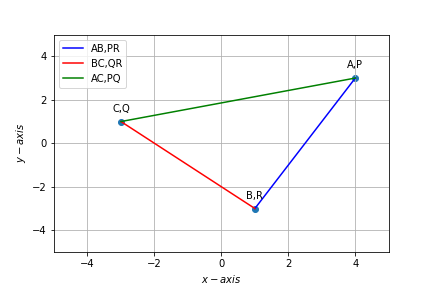
\includegraphics[width=\columnwidth]{triangle.png}
\end{figure}
\end{enumerate}
\end{document}









